%%%%%%%%%%%%%%%%%%%%%%%%%%%%%%%%%%%%%%%%%%%%%%%%%%%%%%%%%%%%%%%%%%%%
%% I, the copyright holder of this work, release this work into the
%% public domain. This applies worldwide. In some countries this may
%% not be legally possible; if so: I grant anyone the right to use
%% this work for any purpose, without any conditions, unless such
%% conditions are required by law.
%%%%%%%%%%%%%%%%%%%%%%%%%%%%%%%%%%%%%%%%%%%%%%%%%%%%%%%%%%%%%%%%%%%%

\documentclass{beamer}
\usetheme[faculty=fi]{fibeamer}
\usepackage{framed}
\usepackage[utf8]{inputenc}
\usepackage{listings}
\usepackage{color}
\usepackage{adjustbox}

\definecolor{dkgreen}{rgb}{0,0.6,0}
\definecolor{gray}{rgb}{0.5,0.5,0.5}
\definecolor{mauve}{rgb}{0.58,0,0.82}
\definecolor{mygray}{gray}{0.3}

\lstset{frame=tb,
	language=Java,
	aboveskip=3mm,
	belowskip=3mm,
	showstringspaces=false,
	columns=flexible,
	basicstyle={\small\ttfamily},
	numbers=none,
	numberstyle=\tiny\color{gray},
	keywordstyle=\color{blue},
	commentstyle=\color{dkgreen},
	stringstyle=\color{mauve},
	breaklines=true,
	breakatwhitespace=true,
	tabsize=3
}
\usepackage[
  main=english, %% By using `czech` or `slovak` as the main locale
                %% instead of `english`, you can typeset the
                %% presentation in either Czech or Slovak,
                %% respectively.
  czech, slovak %% The additional keys allow foreign texts to be
]{babel}        %% typeset as follows:
%%
%%   \begin{otherlanguage}{czech}   ... \end{otherlanguage}
%%   \begin{otherlanguage}{slovak}  ... \end{otherlanguage}
%%
%% These macros specify information about the presentation
\title{
RECOMMENDING WHEN DESIGN TECHNICAL DEBT SHOULD BE SELF-ADMITTED} %% that will be typeset on the
\subtitle{Computer Engineering} %% title page.
\author{Cedric Noiseux}
\date{December 5, 2017}
\defbeamertemplate*{title page}{customized}
{
	\centering
	\begin{framed}
		\usebeamerfont{title}\inserttitle\par
	\end{framed}
	\usebeamerfont{subtitle}\textcolor{white}{\insertsubtitle}\par
	\begin{figure}[t]
		\centering
		
\includegraphics[width=45mm]{resources/logo}
		\vspace{-4mm}
	\end{figure}
	\usebeamerfont{author}\textcolor{white}{\insertauthor}\par
	%\usebeamerfont{institute}\textcolor{lightgray}{\insertinstitute}\par
	\usebeamerfont{date}\textcolor{white}{\insertdate}\par
}
%% These additional packages are used within the document:
\usepackage{ragged2e}  % `\justifying` text
\usepackage{booktabs}  % Tables
\usepackage{tabularx}
\usepackage{tikz}      % Diagrams
\usetikzlibrary{calc, shapes, backgrounds}
\usepackage{amsmath, amssymb}
\usepackage{url}       % `\url`s
\usepackage{listings}  % Code listings
\frenchspacing
\begin{document}
	\begin{darkframes}
		%%%%%%%%%
		% Title Page %
		%%%%%%%%%
		
		\frame{\maketitle}
  
  		%%%%%%%%%%%%%
  		% Table of Content %
  		%%%%%%%%%%%%%
  		
		\begin{frame}[allowframebreaks]
			\frametitle{Table of Contents}
			\tableofcontents[sections={1-2}]
				\framebreak
			\tableofcontents[sections={3-4}]
		\end{frame}
	
		\section{INTRODUCTION}
		
			%%%%%%%%%%%%%%%%%%
			% Concepts and Definitions %
			%%%%%%%%%%%%%%%%%%
	
			\subsection{Concepts and Definitions}	 
			 
				\begin{frame}{Concepts and Definitions}	
					\framesubtitle{Technical Debt (TD)}	
					\begin{block}{Definition}
						TDs are not quite right code which we postpone making it right~\cite{cunn92}. They are temporary and suboptimal solutions or workarounds.
					\end{block}
					\begin{block}{Reasons}
						Quickly fix an issue\\
						Early conception stages\\
						Lack of comprehension, skill or experience	
					\end{block}
				\end{frame}
						
				\begin{frame}{Concepts and Definitions}	
					\framesubtitle{Technical Debt (TD)}	
					\begin{exampleblock}{Types}
						\vspace{1mm}
						\begin{columns}[onlytextwidth]
							\column{.25\textwidth}
							\small 
							Design\\
							Requirement\\
							Code\\
							Test\\
							Documentation\\
							Defect
							\column{.75\textwidth}
							\small
							\alert{Object-Oriented design principles} \\
							\alert{Functional and non functional requirement trade-offs}\\
							\alert{Quality of source code}\\
							\alert{Quality of testing activities}\\
							\alert{Misleading Information}\\
							\alert{Known and possible defects}
						\end{columns}
					\end{exampleblock}	
					\begin{exampleblock}{Impacts}
						Slower conception and execution\\
						Lower maintainability and quality\\
						Higher production cost
					\end{exampleblock}	
				\end{frame}
			
				\begin{frame}{Concepts and Definitions}	
					\framesubtitle{Self-Admitted Technical Debt (SATD)}	
					\begin{block}{Definition}
						SATDs are technical debts which are consciously introduced and explicitly documented by developers.
					\end{block}
					\begin{block}{Characteristics}
						\vspace{1mm}
						\begin{columns}[onlytextwidth]
							\column{.25\textwidth}
							Diffusion\\
							Evolution\\
							Actors
							\column{.75\textwidth}
							\alert{31\% of files contain SATD, 51 instances per system}\\
							\alert{Persistent and increase with time}\\
							\alert{Experienced developers introduce them}
						\end{columns}
					\end{block}
				\end{frame}
			
			%Technical Debts (defintion, impact)
			%Types of Debts
			%Self-Admitted Technical Debts (definition, exploratory study)
						
			%%%%%%%%%%%%%%%%%%%%
			% Elements of the Problematic %
			%%%%%%%%%%%%%%%%%%%%
						
			\subsection{Elements of the Problematic}
			
				\begin{frame}{Elements of the Problematic}	
					\framesubtitle{Self-Admitted Technical Debt (SATD)}	
					\begin{alertblock}{Issues}
						\alert{Weak Performance Results}\\
						\alert{Ineffective Strategies}
						\begin{itemize}
							\small
							\item Code Refactoring
							\item Continuous Tracking
							\item Proactiveness
						\end{itemize}
						\alert{Flawed or Incomplete Approaches}
						\begin{itemize}
							\small
							\item Pattern Matching
							\item Machine Learning with Natural Language Processing
						\end{itemize}
					\end{alertblock}
				\end{frame}
			
%			Low prediction (many FP)
%			Inefficient strategies (refactoring, tracking, etc)
%			Ineficient approaches (pattern matching, ML)

			%%%%%%%%%
			% Objectives %
			%%%%%%%%%
	
			\subsection{Objectives}
			
				\begin{frame}{Objectives}
					\framesubtitle{Main Research Question}	
					\begin{framed}
						\large
						How can we identify and detect \alert{technical debts} in a software project using \alert{source code or features} and known \alert{self-admitted technical debts} with a \alert{machine learning} approach?
					\end{framed}
					\smallskip
					\begin{table}[!b]
						{
							\carlitoTLF % Use monospaced lining figures
							\begin{tabularx}{\textwidth}{*2{>{\centering\arraybackslash}X}@{}}
								\textbf{TEDIOUS} & \textbf{CNN}  \\
								\toprule
								Metrics and Warnings & Source Code \\
								Machine Learners & Neural Network \\
								\bottomrule
							\end{tabularx}
						}
					\end{table}
				\end{frame}
			
				\begin{frame}{Objectives}
					\framesubtitle{Application Objectives}	
					\begin{exampleblock}{Recommendation System}
						To encourage self-admitting technical debts\\
						To ease tracking\\
						To fix issues faster
					\end{exampleblock}		
					\begin{exampleblock}{Complement to existing smell detectors}
						Or use as an alternative
					\end{exampleblock}	
					\begin{table}[!b]
							{
								\carlitoTLF % Use monospaced lining figures
								\begin{tabularx}{\textwidth}{*3{>{\centering\arraybackslash}X}@{}}
									\bottomrule
									\color{dkgreen}\large\textbf{Tracking} & \color{dkgreen}\large\textbf{Managing} & \color{dkgreen}\large\textbf{Improving} \\
								\end{tabularx}
							}
					\end{table}
				\end{frame}
				
				\begin{frame}{Objectives}
					\framesubtitle{Design Objectives}	
					\begin{block}{\small Defining and Extracting Features}
						\small
						\textbf{TEDIOUS} : Metrics and Warnings\\
						\textbf{CNN} : Source Code
					\end{block}
					\begin{block}{\small Identifying SATDs}
	
					\end{block}
					\begin{block}{\small Preprocessing Features}
						\small
						\textbf{TEDIOUS} : Multi-Collinearity, Feature Selection, Normalization, Rebalancing\\
						\textbf{CNN} : Tokenization, Word Embedding
					\end{block}
					\begin{block}{\small Building and Applying Machine Learners}
						\small
						\textbf{TEDIOUS} : Machine Learning Models\\
						\textbf{CNN} : Neural Network
					\end{block}
				\end{frame}
	
			%Research objective (main and 2 application scenarios)
			%Design objectives (5 objectives)
			
		%%%%%%%%%
		% TEDIOUS %
		%%%%%%%%%

	    \section{TEDIOUS}
	    
		    %%%%%%%%%%%%%
		    % Table of Content %
		    %%%%%%%%%%%%%
	    
		    \begin{frame}[allowframebreaks]
		    	\frametitle{Table of Contents}
			    	\begin{enumerate}
			    		\item \textcolor{mygray}{INTRODUCTION}
			    		\begin{enumerate}
			    			\item \textcolor{mygray}{Concepts and Definitions}
			    			\item \textcolor{mygray}{Elements of the Problematic}
			    			\item \textcolor{mygray}{Objectives}
			    		\end{enumerate}
			    	\end{enumerate}
		    		\bigskip
			    	\begin{enumerate}
			    		\item TEDIOUS
			    		\begin{enumerate}
			    			\item Study Definition
			    			\item The Approach
			    			\item Study Results
			    		\end{enumerate}
			    	\end{enumerate}
	    	\end{frame}
    	
    		%%%%%%%%%%%%%
    		% Study Definition %
    		%%%%%%%%%%%%%
	    
	    	\subsection{Study Definition}	
	    	
	    		\begin{frame}{Study Definition}
	    			\framesubtitle{Studied Projects}
	    			\begin{table}[t]
	    				{
	    					\carlitoTLF % Use monospaced lining figures
	    					\scriptsize
	    					\centering
	    					\begin{tabularx}{\textwidth}{l | r r r r | r | r r | r}
   						  		& \multicolumn{4}{c|}{Number of}  & Nb of Com & \multicolumn{2}{c|}{Nb of SATD}  & SATD \\
	    						Project  & F & C & M & Com & $\in$ M & $\notin$ M & $\in$ M & M \% \\
	    						\hline
	    						Ant & 1,113 & 1,575 & 11,052 & 20,325               & 13,359        &  1 & 57 & 0.5\% \\
	    						ArgoUML& 1,922 & 2,579 & 14,346 & 64,393       &  17,722       & 203 & 425  & 2\%\\
	    						Columba & 1,549 & 1,884 & 7,035 & 33,415           & 10,305        & 8 & 418 & 5\%  \\
	    						Hibernate & 2,129 & 2,529 & 17,405 & 15,901 & 9,073        & 21  &  377  &  2\%\\
	    						jEdit & 394 & 889 & 4,785 & 15,468                     &10,894         & 6  & 77  & 2\% \\
	    						jFreeChart & 1,017 & 1,091 & 10,343 & 22,827  & 15,412       &  4  & 1,881  & 18\%\\
	    						jMeter & 1,048 & 1,328 & 8,680 & 19,721                &  12,672      & 95 &  424 & 5\%  \\
	    						jRuby & 970 & 2,063 & 14,163 & 10,599               & 7,809        & 16   & 275  &  2\%\\
	    						Squirrel & 2,325 & 4,123 & 16,648 & 25,216         & 15,574      &35  & 173  & 1\% \\
	    					\end{tabularx}
	    				}
	    			\end{table}
    				\tiny
    				\centering
    				F : Files \hspace{5mm}  C : Classes \hspace{5mm} M : Methods \hspace{5mm} Com : Comments
    				\begin{figure}[t]
    					\centering
    					
\includegraphics[width=20mm]{resources/Hibernate}
    					\hspace{10mm}
    					
\includegraphics[width=5mm]{resources/jEdit}
    					\hspace{10mm} 
    					
\includegraphics[width=15mm]{resources/jMeter}
    					\hspace{10mm} 
    					
\includegraphics[width=15mm]{resources/jRuby}
    				\end{figure}
    			\end{frame}
    		
    			\begin{frame}{Study Definition}
    				\framesubtitle{Research Questions}
    				\centering
    				\begin{block}{RQ1}
    					How does TEDIOUS work for recommending SATD within project?
    				\end{block}
	    			\begin{block}{RQ2}
	    				How does TEDIOUS work for recommending SATD within project?
	    			\end{block}
		    		\begin{block}{RQ3}
		    			How would a method-level smell detector compare with TEDIOUS?
		    		\end{block}
    			\end{frame}
	    	
%	    	Research questions (main and 3 sub-questions)
%	    	9 OOS + Java
%	    	More method-related than class-related
%		    Unbalance

    		%%%%%%%%%%%
			% The Approach %
			%%%%%%%%%%%
		    
		    \subsection{The Approach}
		 
		    \begin{frame}{The Approach}
		    	\framesubtitle{Train and Test Sets}
		    	\begin{figure}[t]
		    		\centering
		    		\fbox{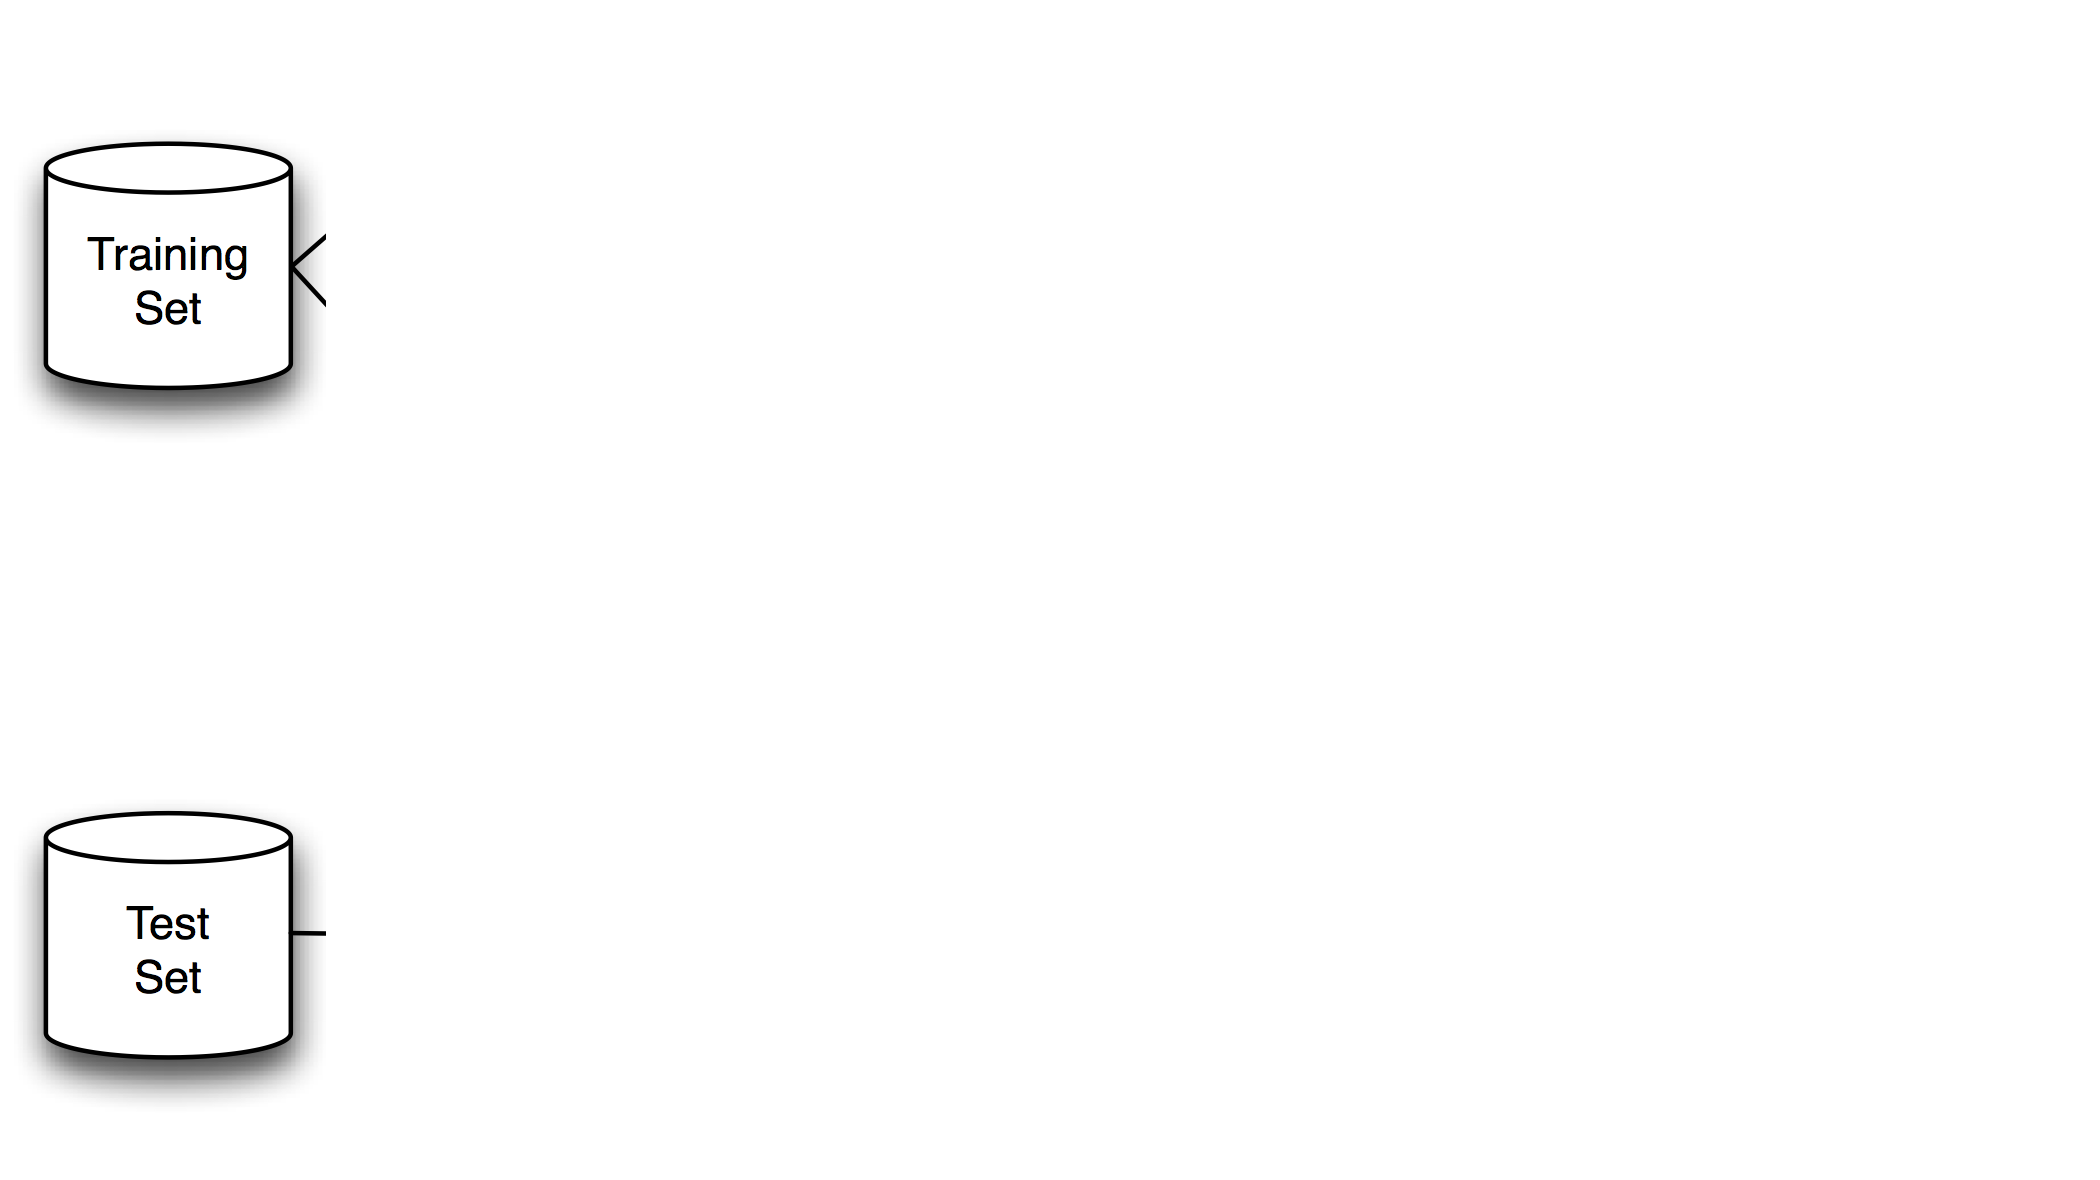
\includegraphics[width=100mm]{resources/tedious-train-test}}
		    	\end{figure}
	    	\end{frame}
    	
    		\begin{frame}{The Approach}
	    		\framesubtitle{SATD Matching}
	    		\begin{figure}[t]
	    			\centering
	    			\fbox{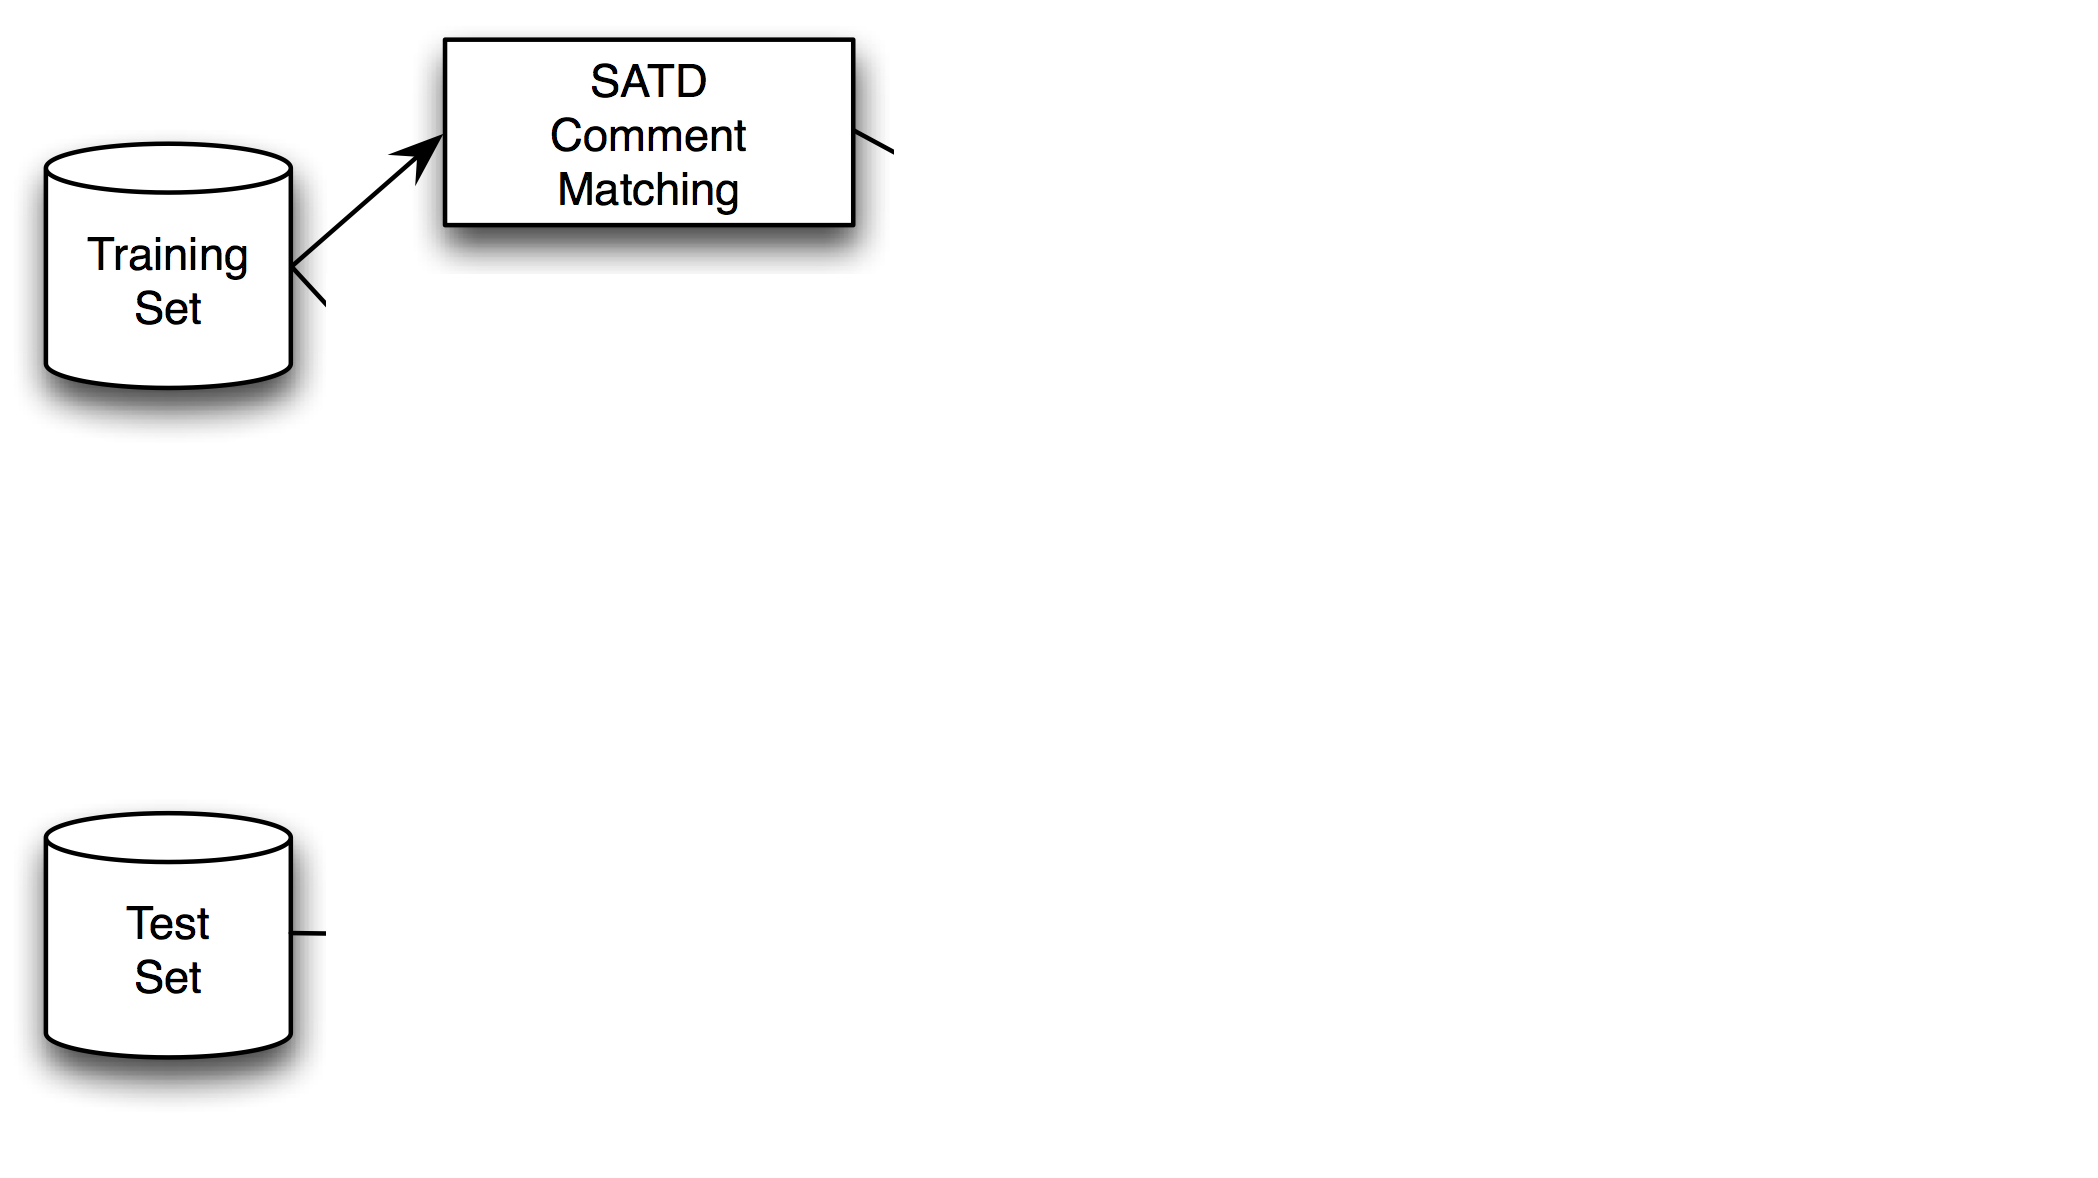
\includegraphics[width=100mm]{resources/tedious-satd}}
	    		\end{figure}
    		\end{frame}
    	
    		\begin{frame}{The Approach}
				\framesubtitle{SATD Matching}    	
				\begin{block}{Identification of Self-Admitted Technical Debt}
					Method-Level\\
					Pattern Matching\\
    				Tagging
    			\end{block}
    		\end{frame}
    	
    		\begin{frame}{The Approach}
	    		\framesubtitle{Features Extraction}
	    		\begin{figure}[t]
	    			\centering
	    			\fbox{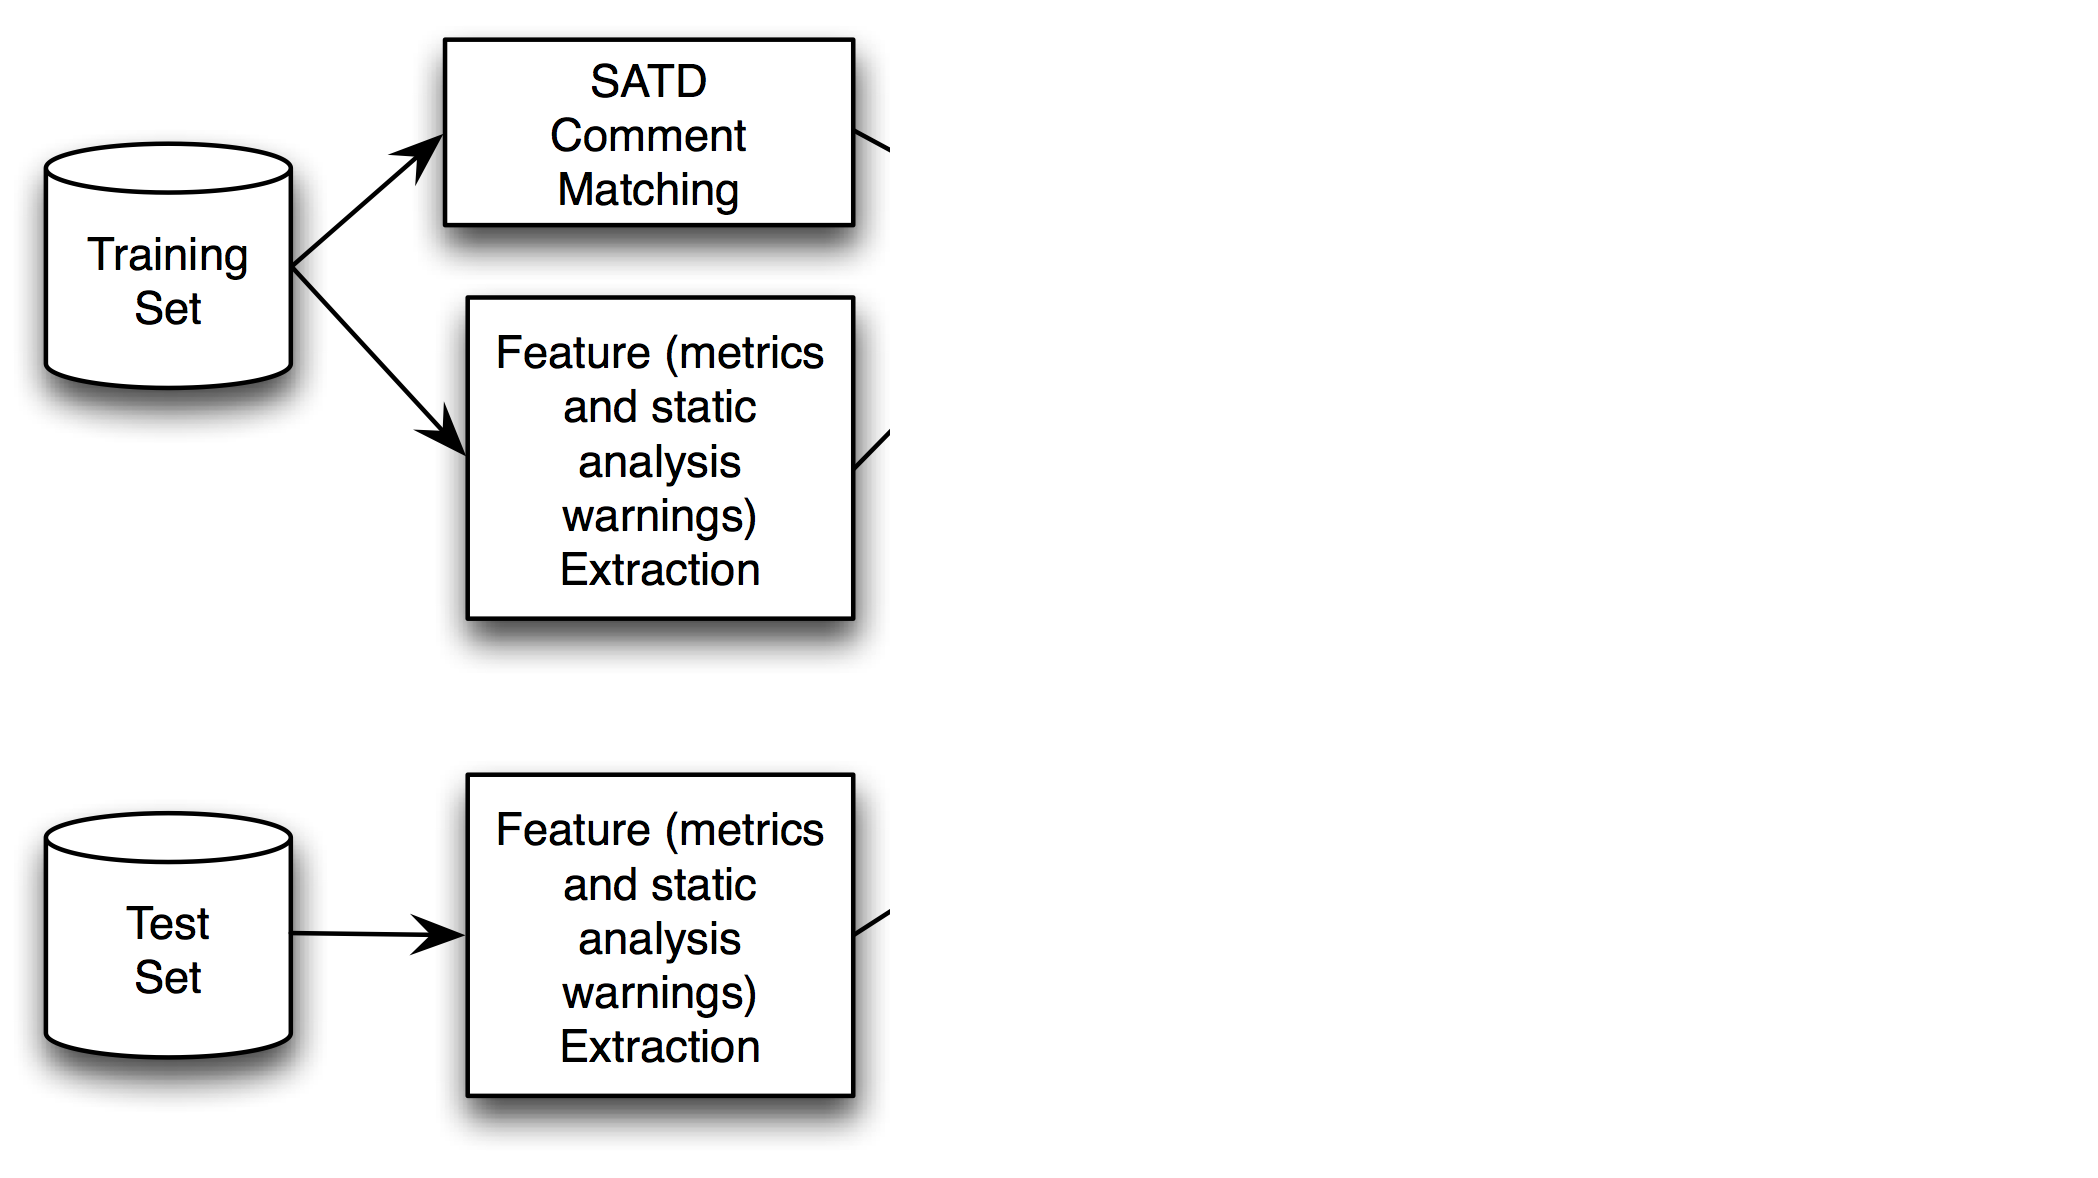
\includegraphics[width=100mm]{resources/tedious-features}}
	    		\end{figure}
	    	\end{frame}
    	
    	    \begin{frame}{The Approach}
    			\framesubtitle{Features Extraction}
    			\begin{figure}[t]
    				\centering
    				\fbox{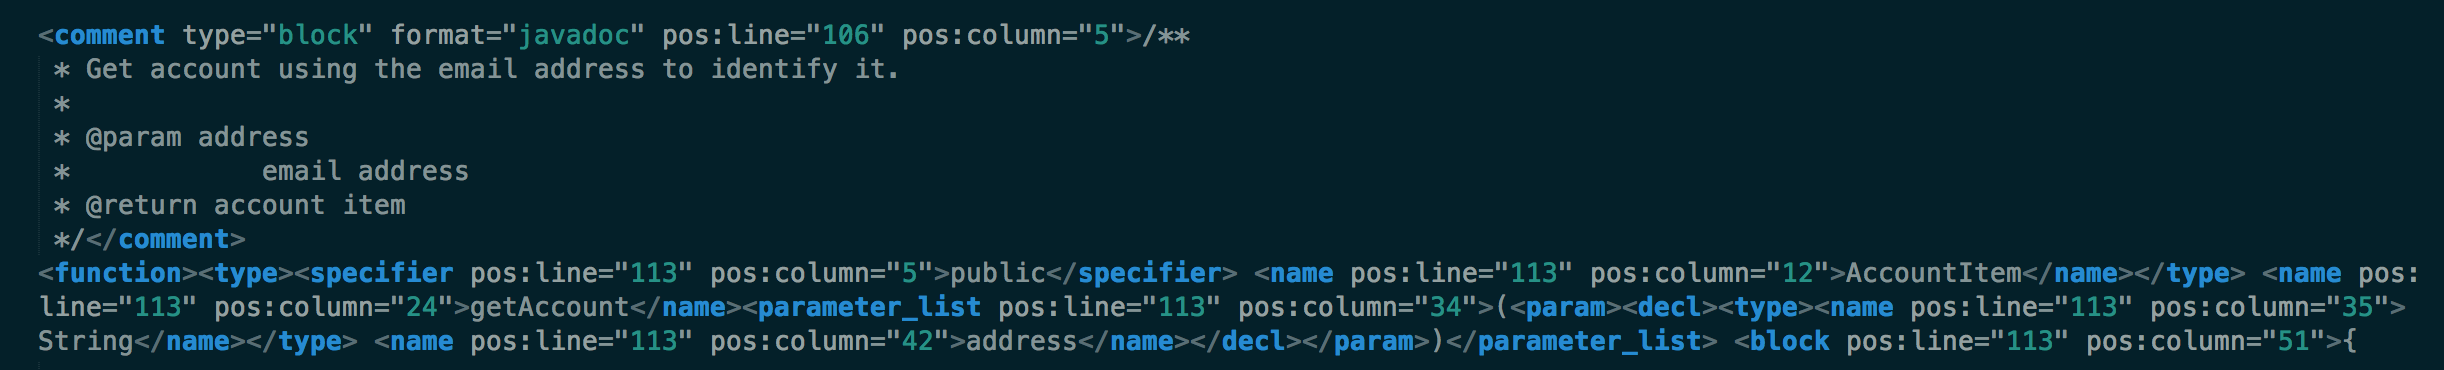
\includegraphics[width=100mm]{resources/xml}}
    			\end{figure}
    			\begin{block}{Source Code Metrics}
    				XML Representation\\
    				Remove SATD Methods\\
    				Compute source code and readability metrics
    			\end{block}
    		\end{frame}
    	
    	    \begin{frame}{The Approach}
    		\framesubtitle{Features Extraction}
    	    	\begin{exampleblock}{\small List of Metrics}
		    		\vspace{1mm}
		    			LOC\\
		    			Nb of Statements\\
		    			Nb of Comments\\
		    			McCabe Cyclomatic Complexity\\
		    			Nb of Expressions
		    			Nb of Passsed Param \\
		    			Nb of Identifiers \\
		    			Nb of Call Sites \\
		    			Nb of Declarations
		    	\end{exampleblock}
	    	\end{frame}
    	
    	    \begin{frame}{The Approach}
		    	\framesubtitle{Feature Preprocessing}
		    	\begin{figure}[t]
		    		\centering
		    		\fbox{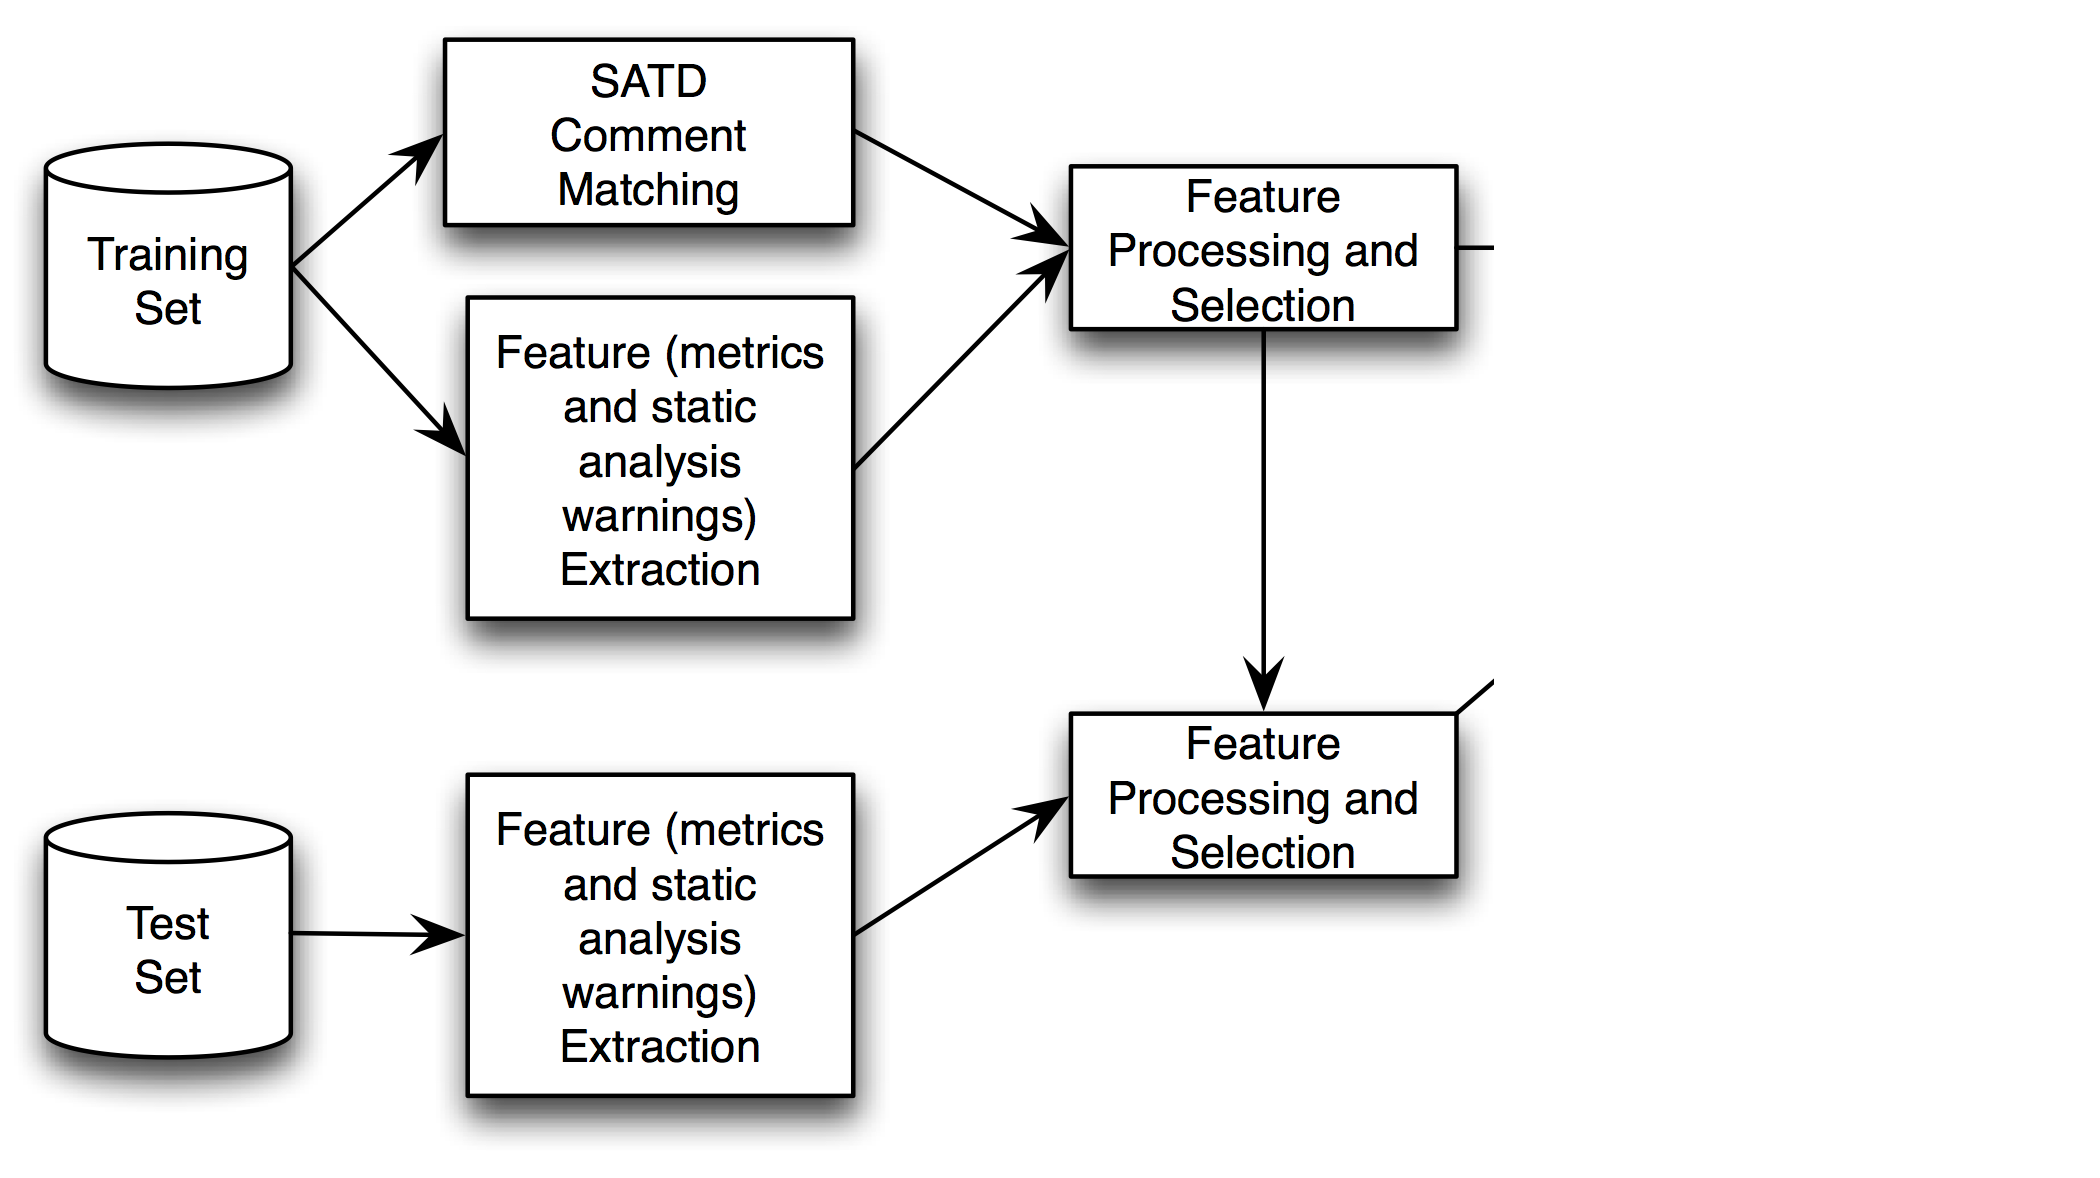
\includegraphics[width=100mm]{resources/tedious-preprocessing}}
		    	\end{figure}
		    \end{frame}
	    
	    
	        \begin{frame}{The Approach}
			    \framesubtitle{Machine Learners}
			    \begin{figure}[t]
			    	\centering
			    	\fbox{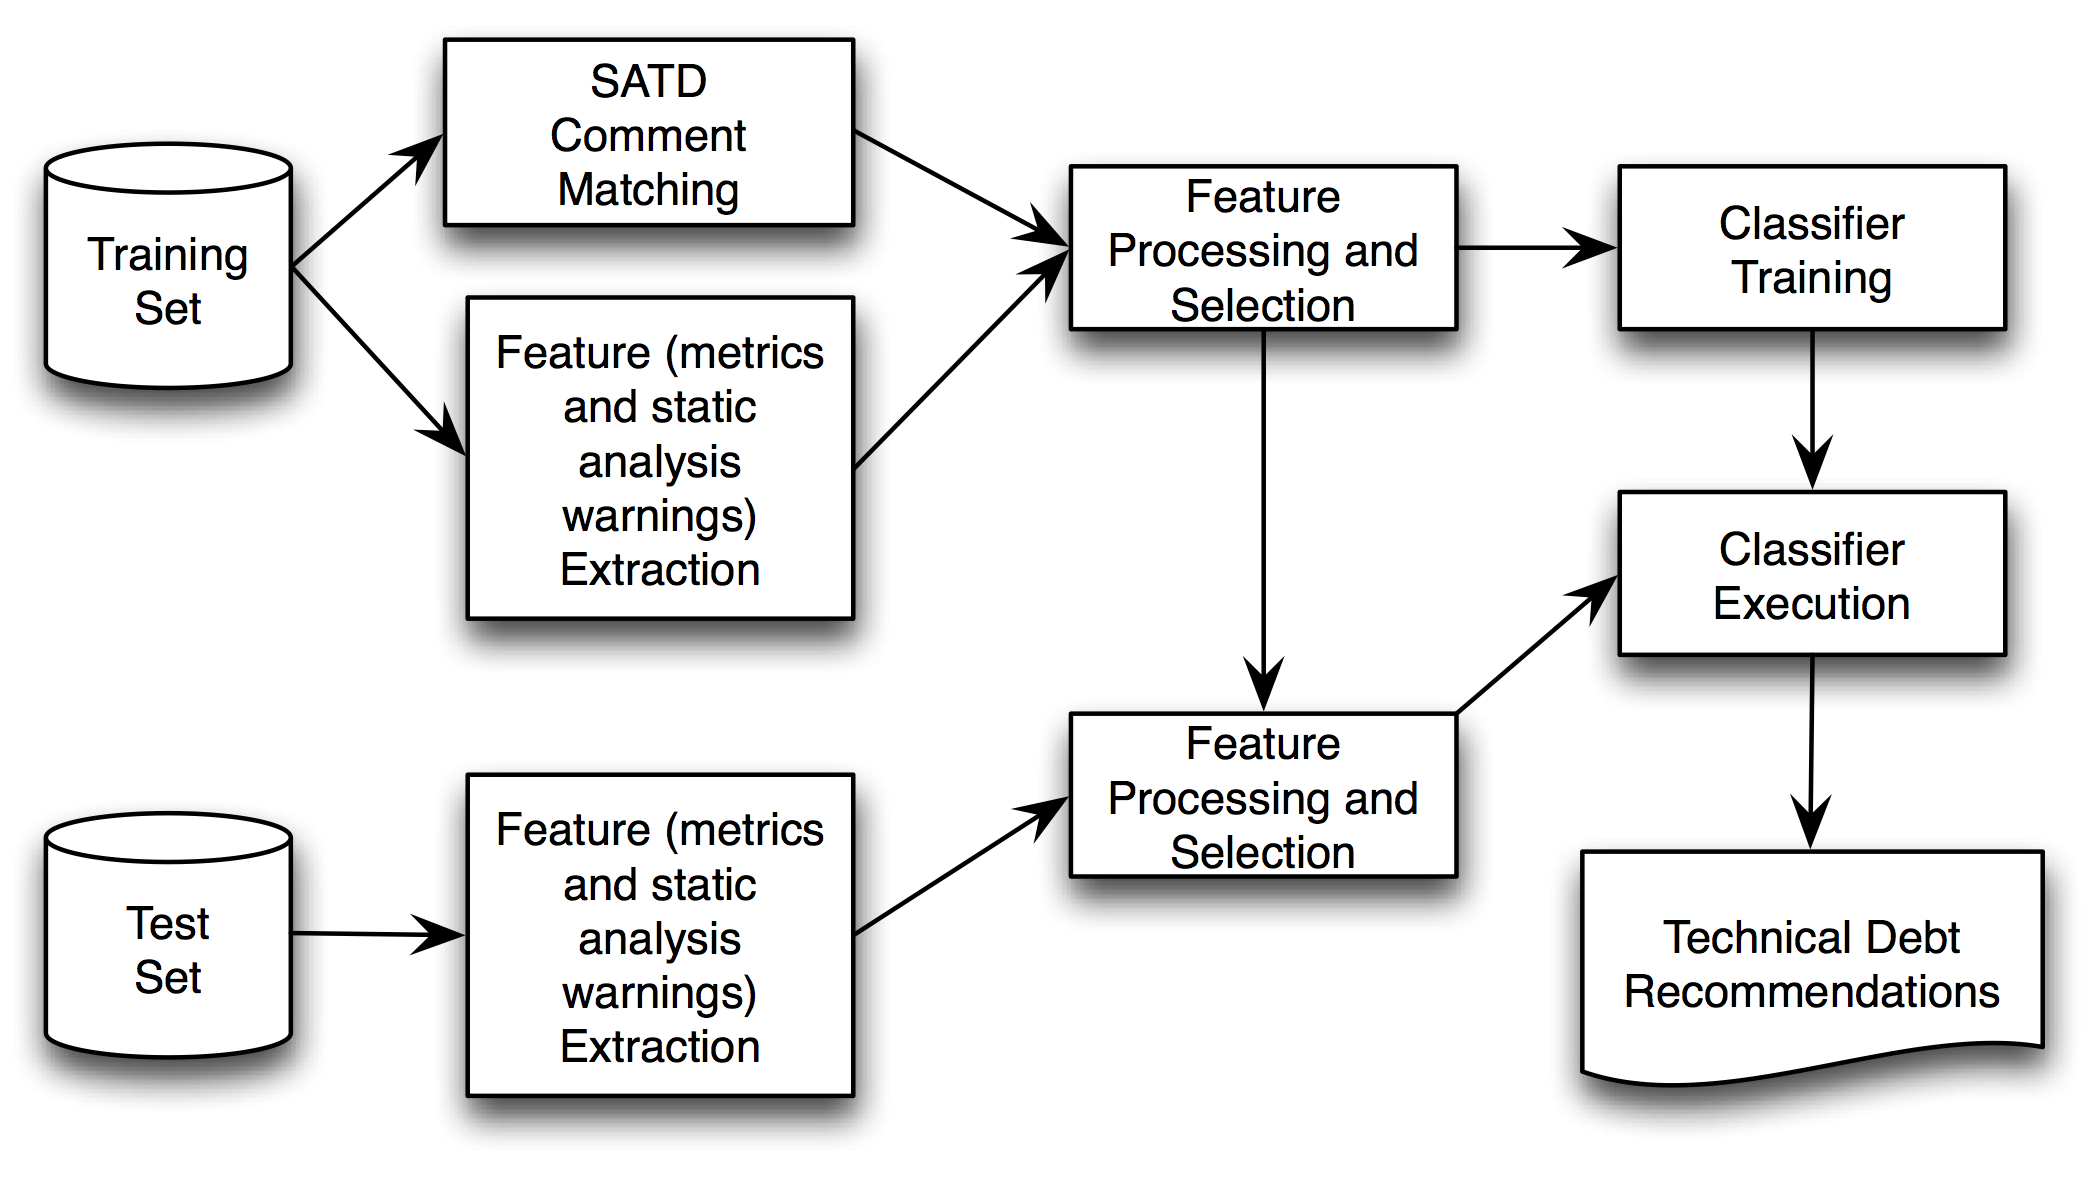
\includegraphics[width=100mm]{resources/tedious-machine-learner}}
			    \end{figure}
		    \end{frame}
		    	
		    Method-level
		    Image du process (separer en differents process et expliquer)
		    	- Training and test sets
		    	- SATD matching
		    	- Features
		    	- Preprocessing
		    	- Building and applying machine learners (training and testing)
		    
		    \subsection{Study Results}
		    
		    Analysis Method
		    Within project performance
		    Cross project performance
		    TEDIOUS vs method level
		    Qualitative analysis
		    
	\end{darkframes}

	\section{CONVOLUTIONAL NEURAL NETWORK}
	
		\subsection{Introduction}
		
		Inspirations (Kim, Dos Santos)
		Description

		\subsection{The Approach}
		
		Method-level
		Image du process (separer en differents process et expliquer)
		- Training and test sets
		- SATD matching
		- Source code
		- Preprocessing/Word Embedings
		- Building and applying machine learners (training and testing)

		\subsection{Study Definition}	
		
		Research questions (main and 3 sub-questions)
		9 OOS + Java
		More method-related than class-related
		Unbalance

		\subsection{Study Results}
		
		Source code comments only
		Source code with comments
		Source code without comments
		Source code partially with comments
			
	\section{CONCLUSION}
	
		\subsection{Threats to Validity}
		
		Construct
		Internal
		Conclusion
		Reliability
		External

		\subsection{Limitations}	
		
		Number of metrics/warning
		Number of LOC
		Process inherent errors
		Default configurations (no real optimizations)
		Generalization of results
		Only in Java
		Performance evaluation can be better for CNN
		
		\subsection{Summary and Future Work}	
	
		TEDIOUS approach
		CNN approach
		Dataset
		TEDIOUS results
		CNN results
		Applicability scenarios
			- Recommendation system
			- Complement to smell detectors
		Improvements
			- Optimization
			- Pattern matching process
			- More examples to train
			- More positive examples
			- More metrics/warnings and source code
			- Other TD types
			- Extend to other languages and domains
			
		\begin{frame}[label=bibliography]{Bibliography}
		\framesubtitle{\TeX, \LaTeX, and Beamer}
		\begin{thebibliography}{9}
			\bibitem{cunn92}
			W~Cunningham.
			\emph{The wycash portfolio management system}.
			dans Addendum to the Proceedings on Object-oriented Programming Systems, Languages, and Applications (Addendum), s\'{e}rie OOPSLA ’92, New York, NY, USA: ACM, 1992, pp 29–30, DOI: 10.1145/157709.157715. En ligne: http://doi.acm.org/10.1145/157709.157715.
			\end{thebibliography}
		\end{frame}
	
\end{document}
